%!TEX root = ../thesis.tex
%*******************************************************************************
%****************************** Second Chapter *********************************
%*******************************************************************************

\chapter{Parameter Estimation for Hidden Markov Models}

\ifpdf
    \graphicspath{{Chapter2/Figs/Raster/}{Chapter2/Figs/PDF/}{Chapter2/Figs/}}
\else
    \graphicspath{{Chapter2/Figs/Vector/}{Chapter2/Figs/}}
\fi

\section{ Expectation–Maximization algorithm}

Also abbreviated as \textbf{EM algorithm} is an iterative approach for maximum likelihood estimates of model parameters. 
It is used in situations where incomplete data are present therefore a part of a complete data set is hidden, 
and we may not be able to apply straightforward analytical procedures for computing maximum likelihood estimates as in a 
case of complete data. EM algorithm introduce further below is mainly based on the work of \cite{Dempster1977}.

In other words, we want to find the best estimate of the parameters for which the observed sequence of emissions is the most likely. 
This is of great importance and efficiency in Hidden Markov models where we have a space of emissions and states, where  emissions 
are observed and states are hidden. We also know that the state space is in our case finite, and therefore we can enumerate all possible states.

Let us also denote $\theta \in \Theta$ which is a vector of parameters belonging to parameter space $\Theta$. 
The aim of EM algorithm is essentially to find the "best" estimate of $\theta$ that maximizes the likelihood function $L(\theta|\textbf{Y})$, 
this is well known as Maximum likelihood estimate (MLE) that leads to $\hat{\theta}_{MLE}$. 

\subsection*{Complete data}

To apply the non-iterative approach for complete data, let us consider daily log-returns of BTC/USDT trading pair in past 5 years. 
Plotting the histogram we conclude that the log-returns may asymptotically follow normal distribution. 
Since the probability density function in such case is unimodal and has only one global maximum, 
the logarithmic transformation of likelihood function conveniently converts multiplication to addition with the 
preservation of global maximum to be optimized by taking the partial derivative w.r.t.\ each parameter. 
First, we formulate the likelihood function of two-parametric normal distribution $\mathcal{N}(\mu,\sigma^2)$ given an observed sequence 
of log-returns $\textbf{Y} = \{y_1,\ldots,y_T\}$ where $T \in \mathbb{N}$:
 
\begin{equation}
    L(\mu,\sigma^2|\textbf{Y}) = \prod_{t=1}^{T} \frac{1}{\sqrt{2\pi \sigma^2}} e^{-\frac{1}{2} \frac{{(y_t-\mu)}^2}{\sigma^2}}
\end{equation}

\begin{equation}
    \ell(\mu,\sigma^2|\textbf{Y}) = \sum_{t=1}^{T} \ln L(\mu,\sigma^2|y_t) 
\end{equation}

where $x_1,\ldots,x_N$ is a vector of log-returns of length N and $\mu$ and $\sigma^2$ are parameters to be estimated. 

\begin{equation}
    \ell(\mu,\sigma^2|\textbf{Y}) = -\frac{T}{2} \ln(2 \pi) - \frac{T}{2} \ln(\sigma^2) - \frac{1}{2 \sigma^2} \sum_{t=1}^{T} {(y_t - \mu)}^2
\end{equation}

If we now take the partial derivative w.r.t.\ the parameter $\mu$ and $\sigma^2$ and set it to zero we obtain the ML estimate of the 
parameters as follows:

\begin{gather} 
\frac{\partial \ell(\mu,\sigma^2|\textbf{Y})}{\partial \mu}  = \frac{1}{\sigma^2} (\sum_{t=1}^{T} y_t - T\mu) \nonumber \\
0 = \frac{1}{\sigma^2} (\sum_{t=1}^{T} y_t - T\mu) \nonumber\\
\hat{\mu}_{MLE} = \frac{\sum_{t=1}^{T} y_t}{T} \label{eq:MLEmu}
\end{gather}

\begin{gather} 
\frac{\partial \ell(\mu,\sigma^2|\textbf{Y})}{\partial \sigma^2}  = -\frac{T}{\sigma}+ \frac{1}{\sigma^3} \sum_{t=1}^{T} {(y_t - \mu)}^2 \nonumber\\
0 = -\frac{T}{\sigma}+ \frac{1}{\sigma^3} \sum_{t=1}^{T} {(y_t - \mu)}^2 \nonumber\\
\hat{\sigma}_{MLE}^2 = \frac{\sum_{t=1}^{T} {(y_t - \mu)}^2}{T} \label{eq:MLEsigma} 
\end{gather}

Inserting observed data $\textbf{Y}$ into Equation \ref{eq:MLEmu} and \ref{eq:MLEsigma}, ML estimate of $\mu$ is 0.003 and $\sigma^2$ 
0.042 respectively. Histogram with curve TODO.

\subsection*{Incomplete data}

Although the assumption of complete data simplifies the analytical procedure of calculating the ML estimate in closed form, 
it is not easily applicable in case of incomplete data, i.e. when some information is latent which is particularly true for Hidden Markov Models. 
The alternative for the likelihood function of the complete data is therefore to use a joint probability of observed and hidden part of the data to 
obtain a marginal probability by summing over all possible hidden states $i \in I$. 

\begin{equation} \label{eq:loglike}
\ell(\theta|\textbf{Y}) = \sum_{t=1}^{T} \ln \mathbb{P}(Y_t= y_t|\theta) = \sum_{t=1}^{T} \ln \sum\limits_{i=1}^N \mathbb{P}(Y_t= y_t,X_t=i|\theta)
\end{equation}

Since the natural logarithm is strictly monotonic increasing function the value of $\theta$ maximizes the log-likelihood as well as the 
likelihood function. Simply, the EM algorithm iterates over possible values of $\theta$ to find the best estimate in terms of log-likelihood difference, 
i.e.\ until convergence criterion is satisfied:

\begin{equation} \label{eq:conv}
\frac{|\ell(\theta^{(k)}|\textbf{Y}) - \ell(\theta^{(k-1)}|\textbf{Y})|}{|\ell(\theta^{(k)}|\textbf{Y})|} \leq \epsilon 
\end{equation}

where the current estimate of $\theta$ for k-th iteration is denoted with $(k)$ superscript 
and the convergence threshold $\epsilon$. 

Since the log-likelihood function in Equation \ref{eq:loglike} is not analytically tractable and involves logarithm of a sum,
we need to find an alternative approach to estimate the parameters.
It is, however, possible to introduce several assumptions that will eventually suffice in providing 
direct iterative solution to the optimization problem. Let us first construct a lower bound for the 
marginal likelihood in Equation \ref{eq:loglike}. 

We introduce density function $q(x)$ called "averaging distribution" and start by multiplying 
the joint likelihood by $\frac{q(x)}{q(x)}$. Such expression will allow for a construction of 
artificial weights and with the use of Jensen's inequality:

\begin{align}
    \sum_{t=1}^{T} \ln \sum_{i=1}^{N} q(X_t = i) \frac{p(Y_t=y_t, X_t = i|\theta)}{q(X_t = i)} \geq& \sum_{t=1}^{T} \sum_{i=1}^{N} q(X_t = i) \ln \frac{p(Y_T =y_t, X_t = i|\theta)}{q(X_t = i)} \\
    \ell(\theta|\textbf{Y}) \geq& L(\theta,q|\textbf{Y}), \quad \forall q \in Q
\end{align}

where $Q$ is a set of all possible probability distributions.

The constructed lower bound $L(\theta,q|\textbf{Y})$ can be factorized into the expectation 
of the joint log-likelihood w.r.t to distribution $q(x)$ and entropy $H(q)$:

\begin{equation}
    L(\theta,q|\textbf{Y}) = E_{q(x)} [\ln p(\textbf{X},\textbf{Y}|\theta)] + H(q)
\end{equation}

where $E_{q(x)} [\ln p(X,Y|\theta)]$ is called the \textbf{complete data log-likelihood function} (or Q-function).
Moreover, $H(q)$ is a constant and does not depend on the parameter $\theta$ and therefore can be omitted from the
optimization problem. Therefore, decoupling the log-likelihood function into two parts, we obtain the following expression:

\begin{equation}
    \ell(\theta|\textbf{Y}) = E_{q(x)} [\ln p(\textbf{X},\textbf{Y}|\theta)] + D_{KL} (q(\textbf{X}) || p(\textbf{X}| \textbf{Y},\theta))
\end{equation}

where $D_{KL}$ is the \textit{Kullback-Leibler divergence} between the distribution $q(x)$ and the posterior distribution $p(\textbf{X}|\textbf{Y},\theta)$.
The Kullback-Leibler divergence is a measure of dissimilarity between two probability distributions, and we may interpret it as a geometrical statistical distance.
It is also asymmetric and non-negative, and it is zero if and only if the two probability measures are equal which is a result of \textit{Gibb's inequality}.
These properties are of great importance in the EM algorithm because in order to minimize the distance between the two distributions as described above,
we need to set the distribution $q(x)$ equal to the posterior distribution $p(\textbf{X}|\textbf{Y},\theta)$.

This, first step of the algorithm abbreviated as \textbf{E-step} results in estimating the function $q$ for a $\theta^{k}$, given the k-th iteration of EM algorithm, 
that maximizes the lower bound $L(\theta,q|\textbf{Y})$. s.t. the "distance" from the lower bound to log-likelihood function $\ell(\theta|\textbf{Y})$ is minimized:

\begin{equation}
    q^{k+1} = \underset{q \in Q}{\arg\max} L(\theta^{(k)},q|\textbf{Y}) = p(\textbf{X}|\textbf{Y},\theta^{(k)})
\end{equation}

In other words, we want to minimize distance between the complete data log-likelihood function $L(\theta,q|\textbf{Y})$ and incomplete data $\ell(\theta|\textbf{Y})$ 
with respect to function $q(x)$. Kullback-Leibler divergence (hereafter KL divergence) measure is commonly used in image or signal processing 
in calculation of the expected excess surprise from using $q$ as a probability distribution for our model given that the true or actual 
probability distribution is $p$. Substantially, the measure is a difference of cross-entropy denoted by $H(p,q)$ and entropy by $H(p)$ which 
is also always non-negative as a result of Gibb's inequality.

\begin{align}
D_{KL} (p || q) &= \sum_{X} p(x) \ln \frac{p(x)}{q(x)} \\
& = \sum_{x} p(x) \ln \frac{1}{q(x)} - \sum_{x} p(x) \ln \frac{1}{p(x)} \\
& = H(p,q) - H(p)
\end{align}

More rigorously, we have only defined the lower bound for the complete data log-likelihood function using arbitrary probability function $q(x)$, 
but the deeper examination of the lower bound with the use of KL divergence directly yields the choice of marginal posterior 
distribution $p(\textbf{X}|\textbf{Y},\theta)$ for the probability function $q(x)$:

\begin{align}
l(\theta,q|\textbf{Y}) &= \sum_{i=1}^{N} q(X = i) \ln \frac{p(X = i,\textbf{Y}|\theta)}{q(X = i)} \\
& = \sum_{i=1}^{N} q(X = i) \ln \frac{p(X = i|\textbf{Y},\theta) p(|\textbf{Y}, \theta)}{q(X = i)} \\
& = \sum_{i=1}^{N} q(X = j) \ln \frac{p(X = i|\textbf{Y},\theta)}{q(X = i)} + \sum_{i=1}^{N} q(X = i) \ln p(X|\textbf{Y},\theta)\\
& = -D_{KL}(q(X)||p(X|\textbf{Y},\theta)) + E_{q(x)} [\ln p(\textbf{X},\textbf{Y}|\theta)]
\end{align}

Now we see that the statistical distance between the two likelihood functions is determined solely by the KL divergence.
 In order to find the minimal distance, ideally distance of zero length, we simply set the function $q(x)$ equal to the $p(z|X,\theta)$.

To visualize the EM algorithm, refer to Figure \ref{fig:Loglike} where red curve is the log-likelihood function $\ell(\theta|\textbf{Y})$
and notice that the blue curve already represents the lower bound
after the first iteration of E-step yielding $q^{(k)}$ as a solution. Afterwards parameter estimates of $\theta^{(k)}$ are obtained as part of the M-step 
s.t. the next iteration of E-step can be performed, and the lower bound is maximized again represented by the green curve.


Until now, we have considered the optimal manner in which we compute the conditional expectation $E_{Z|X,\theta_n} [\ln P(X,z|\theta)]$ by 
finding the appropriate function $q$. Next step is, as is typical for coordinate descent, selection of parameter $\theta_{k+1}$ by fixing 
the function $q^{k+1}$ from E-step. The goal of M-step is to:

\begin{equation}
\theta^{k+1} = \underset{\theta}{\arg\max} L(\theta, q^{k+1})
\end{equation}

\begin{figure}[ht]

\begin{center}
	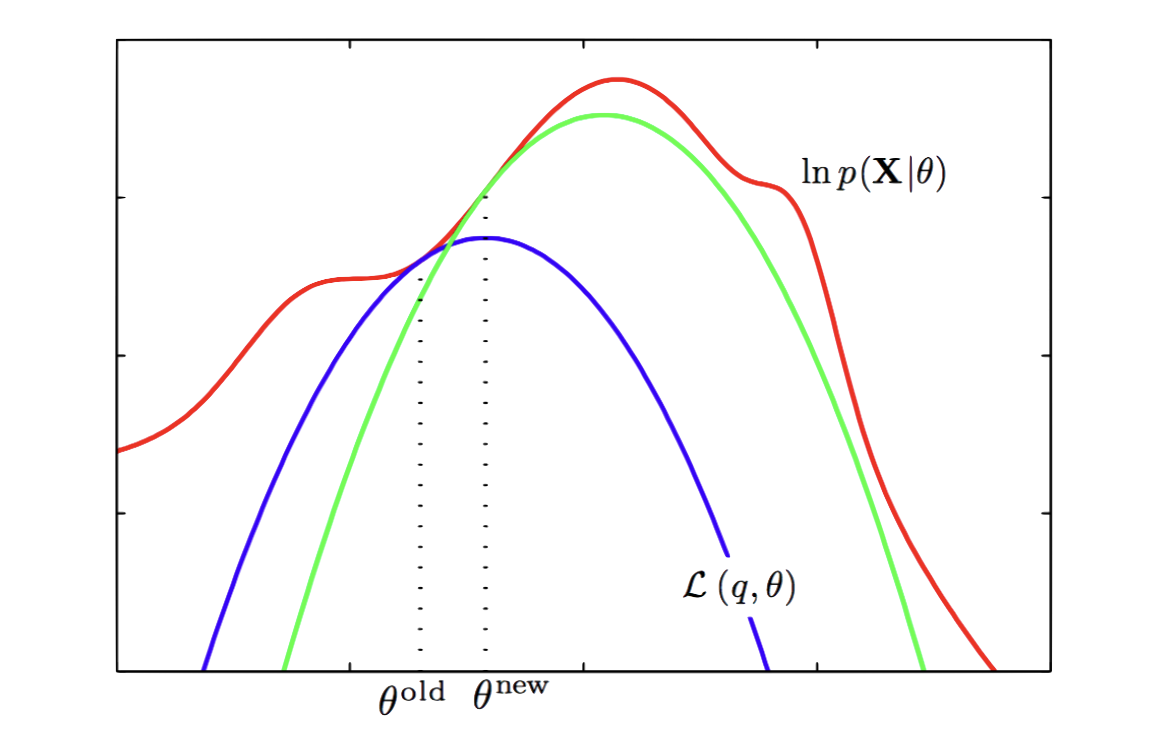
\includegraphics[width=0.9\textwidth]{Figs/Loglike.png}
\end{center}

\caption{\textit{E-step as a problem of minimization of KL divergence represented as a gap between two likelihood functions}}
\label{fig:Loglike}
\end{figure}

\noindent Thus, as a summarization, the EM algorithm involves two steps:

\begin{itemize}
\item[1)] \textbf{Expectation step (E-step)} - choose a function q, i.e.\ probability distribution, that maximizes $L(\theta, q)$, which may be also viewed as computing the conditional expectation $E_{Z|X,\theta_n} [\log p(X,z|\theta)]$ based on the current parameter of $\theta$.
\item[2)] \textbf{Maximization step (M-step)} - estimating the parameter $\theta_{k+1}$ that maximizes the conditional expectation $E_{Z|X,\theta_n} [\log p(X,z|\theta)]$.
\end{itemize}

Both of these steps are repeated until convergence criterion given by Equation \ref{eq:conv} is attained assuming fixed tolerance $\epsilon$.

\subsection{Forward and Backward algorithm}

While given a sequence of emissions denoted by $\textbf{Y}, = \{y_0,y_1,\ldots,y_T\}$ and a model parameter vector $\theta = (\textbf{A},\textbf{B},\textbf{p})$, 
we need to express the likelihood function under the model constraints as follows:
\begin{align}
    \mathcal{L}( \theta| \textbf{Y}) & = \prod\limits_{t=0}^T \sum\limits_{i=1}^N  \mathbb{P}(Y_t = y_t, X_t = i| \theta) \\
                                     & = \prod\limits_{t=0}^T \sum\limits_{i=1}^N  \mathbb{P}(Y_t = y_t | X_t = i, \theta) \mathbb{P}(X_t=i|\theta)
\end{align}

where $N$ denotes a number of hidden states. As in the previous chapter, we need to rather work with log-likelihood function which is more analytically convenient 
and allows us to avoid numerical underflow:

\begin{equation} \label{eq:loglikeFB} 
    l(\theta| \textbf{Y}) = \sum\limits_{t=0}^T \ln \sum\limits_{i=1}^N  \mathbb{P}(Y_t = y_t , X_t = i|\theta)
\end{equation}

As we can see, the summation is nested, and therefore we cannot simply swap the order of summation and logarithm. Therefore, we need to find a way to compute the log-likelihood function 
in a more efficient way. Our goal is to estimate the posterior distribution of the hidden states given the observed sequence of emissions $p(\textbf{X}|\textbf{Y},\theta)$
that helps us to compute the expectation of the complete data log-likelihood function.

The summation in Equation \ref{eq:loglikeFB} refers to all possible permutations of the sequence of hidden states \textbf{X} 
which implies that we would have $N^T$ possible sequences as seen in Figure \ref{fig:trellis}. Furthermore, in order to calculate $\mathcal{L}( \theta| \textbf{Y})$ we have $2TN^T$ 
operations which is also exponential in T and not feasible for real application. As opposed to brute-force 
computation described above, we take a use of \textbf{Forward} and \textbf{Backward} pass to address \textbf{E-step} of the EM algorithm.

\begin{figure}[htbp]
    \begin{center}
    \begin{tikzpicture}[]
    % 1st column
    \node               at (0,6) {$t=0$};
    \node[state] (s1_1) at (0,5) {$S_1$};
    \node[mainstate] (s2_1) at (0,3.5) {$S_2$};
    \node[state] (s3_1) at (0,2) {$\ldots$};
    \node[state] (s4_1) at (0,0.5) {$S_N$};
    \node at (0,-0.5) {$y_0$};    % 2nd column
    \node               at (2,6) {$t=1$};
    \node[mainstate] (s1_2) at (2,5) {$S_1$}
        edge[lightedge] (s1_1)
        edge[lightedge] (s2_1)
        edge[lightedge] (s3_1)
        edge[lightedge] (s4_1);
    \node[state] (s2_2) at (2,3.5) {$S_2$}
        edge[lightedge] (s1_1)
        edge[lightedge] (s2_1)
        edge[lightedge] (s3_1)
        edge[lightedge] (s4_1);
    \node[state] (s3_2) at (2,2) {$\ldots$}
        edge[lightedge] (s1_1)
        edge[lightedge] (s2_1)
        edge[lightedge] (s3_1)
        edge[lightedge] (s4_1);
    \node[state] (s4_2) at (2,0.5) {$S_N$}
        edge[lightedge] (s1_1)
        edge[lightedge] (s2_1)
        edge[lightedge] (s3_1)
        edge[lightedge] (s4_1);
    \node at (2,-0.5) {$y_1$};
    % 3rd column
    \node               at (4,6) {$t=2$};
    \node[mainstate] (s1_3) at (4,5) {$S_1$}
        edge[lightedge]  (s1_2)
        edge[lightedge] (s2_2)
        edge[lightedge] (s3_2)
        edge[lightedge] (s4_2);
    \node[state] (s2_3) at (4,3.5) {$S_2$}
        edge[lightedge] (s1_2)
        edge[lightedge] (s2_2)
        edge[lightedge] (s3_2)
        edge[lightedge] (s4_2);
    \node[state] (s3_3) at (4,2) {$\ldots$}
        edge[lightedge] (s1_2)
        edge[lightedge] (s2_2)
        edge[lightedge] (s3_2)
        edge[lightedge] (s4_2);
    \node[state] (s4_3) at (4,0.5) {$S_N$}
        edge[lightedge] (s1_2)
        edge[lightedge] (s2_2)
        edge[lightedge] (s3_2)
        edge[lightedge] (s4_2);
    \node at (4,-0.5) {$y_2$};
    % 4th column
    \node               at (6,6) {$t=3$};
    \node[mainstate] (s1_4) at (6,5) {$S_1$}
        edge[lightedge]  (s1_3)
        edge[lightedge] (s2_3)
        edge[lightedge] (s3_3)
        edge[lightedge] (s4_3);
    \node[state] (s2_4) at (6,3.5) {$S_2$}
        edge[lightedge] (s1_3)
        edge[lightedge] (s2_3)
        edge[lightedge] (s3_3)
        edge[lightedge] (s4_3);
    \node[state] (s3_4) at (6,2) {$\ldots$}
        edge[lightedge] (s1_3)
        edge[lightedge] (s2_3)
        edge[lightedge] (s3_3)
        edge[lightedge] (s4_3);
    \node[state] (s4_4) at (6,0.5) {$S_N$}
        edge[lightedge] (s1_3)
        edge[lightedge] (s2_3)
        edge[lightedge] (s3_3)
        edge[lightedge] (s4_3);
    \node at (6,-0.5) {$y_3$};
    % 5th column
    \node               at (8,6) {$t=5$};
    \node[mainstate] (s1_5) at (8,5) {$S_1$}
        edge[lightedge]  (s1_4)
        edge[lightedge] (s2_4)
        edge[lightedge] (s3_4)
        edge[lightedge] (s4_4);
    \node[state] (s2_5) at (8,3.5) {$S_2$}
        edge[lightedge] (s1_4)
        edge[lightedge] (s2_4)
        edge[lightedge] (s3_4)
        edge[lightedge] (s4_4);
    \node[state] (s3_5) at (8,2) {$\ldots$}
        edge[lightedge] (s1_4)
        edge[lightedge] (s2_4)
        edge[lightedge] (s3_4)
        edge[lightedge] (s4_4);
    \node[state] (s4_5) at (8,0.5) {$S_N$}
        edge[lightedge] (s1_4)
        edge[lightedge] (s2_4)
        edge[lightedge] (s3_4)
        edge[lightedge] (s4_4);
    \node at (8,-0.5) {$y_4$};
    \end{tikzpicture}
    \end{center}
    \caption{Trellis of the emission sequence $\{y_0$, \ldots,$y_4\}$ for T=4. Each node represents a state $S_i$ and each arc represents a transition from one state to another. The number of possible paths is $N^T$. }
    \label{fig:trellis}
    \end{figure}

\subsubsection{Forward algorithm}

Previous introduction required huge amounts of calculations that were essentially unnecessary and redundant. 
Each sequence can be decomposed into multiple subsequences which are shared among different sequences and do not need to be recomputed again. 
These subsequences can be represented by a trellis as shown in Figure \ref{fig:trellis} With a help of such diagram we may imagine recording the probability of 
distinct subsequences at each time step. In other words, we wish to compute a joint probability while taking advantage 
of the conditional emission independence of $Y_t$ given $X_t$ with respect to the remaining elements of the emission sequence. 
Moreover, due to Markov memoryless property, $X_t$ depends only on $X_{t-1}$. Let us now define the forward probability variable $\alpha_t(i)$ as follows:

\begin{equation}
    \alpha_t(i) = \mathbb{P}(Y_t = y_t, Y_{t-1} = y_{t-1},\ldots, Y_0 = y_0 , X_t = i| \theta)
\end{equation}

Which we may also define as the probability of being in state i at time t after having observed the sequence $\{y_0,x_1,\ldots,y_t\}$. 
The calculation therefore results in recursively summing the incoming arcs at trellis nodes:

\begin{align}
    \alpha_t(i) &= \mathbb{P}(Y_t = y_t, Y_{t-1} = y_{t-1},\ldots, Y_0 = y_0 , X_t = i| \theta) \\ \nonumber
                &= \mathbb{P}(Y_t = y_t | X_t = i, \theta) \mathbb{P}(Y_{t-1} = y_{t-1},\ldots, Y_0 = y_0 , X_t = i| \theta)  \\ \nonumber
                &= \mathbb{P}(Y_t = y_t | X_t = i, \theta) \sum\limits_{j = 1}^N \mathbb{P}(X_t = i| X_{t-1}=j,\theta) \alpha_{t-1}(j)\\ \nonumber
                &= b_i(y_t) \sum\limits_{j=1}^N a_{ji} \alpha_{t-1}(j)
\end{align}

where we ought to initialize forward variable at time $t=0$ as $\alpha_0(i)= p_i b_i(y_0)$. 
The recursive relationship is repeated until termination at time T where it holds that:

\begin{equation} \label{eq:loglikeF}
    \sum_{i=1}^N \alpha_T(i) = \mathcal{L}( \theta| \textbf{Y})
\end{equation} 

Resulting algorithm requires time complexity of $O(TN^2)$\footnote{The O(n) symbol represents Big O notation, 
a convention in computer science to describe how an algorithm's running time or space needs grow as the input size increases. 
O(n) indicates that the growth is linear in relation to the input size n.} 
which is a significant improvement from the brute force approach with complexity of $O(2TN^T)$.

\subsubsection{Backward algorithm}

While computing the backward probability variable denoted as $\beta_t(i)$ we assume the reversed iterative procedure. 
Let us define the backward probability $\beta$ variable as:

\begin{align}
\beta_t(i)  &= \mathbb{P}(Y_{t+1} = y_{t+1}, Y_{t+2} = y_{t+2},\ldots, Y_T = y_T| X_t = i, \theta) \\ \nonumber
            &= \sum_{i,j}^N \mathbb{P}(Y_{t+1} = y_{t+1}, Y_{t+2} = y_{t+2},\ldots, Y_T = y_T,X_{t+1} = j | X_t = i, \theta)  \\ \nonumber
            &= \sum_{i,j}^N \mathbb{P}(Y_{t+1} = y_{t+1}| X_{t+1} = j) \mathbb{P}(X_{t+1} = j | X_t = i, \theta) \\ \nonumber
            & \mathbb{P}(Y_{t+2},\ldots,Y_{t-1},Y_t|X_{t+1}=j)  \\ \nonumber
            &= \sum_{j=1}^N b_j(y_{t+1})a_{ij} \beta_{t+1}(j)
\end{align}

As for forward algorithm, the recursive computation is very similar, the only differences are in the fact that we are going backwards in time using our emission sequence 
while also accounting for the emission probabilities at previous step. Effectively, there are 3 main steps:

\begin{itemize}
\item[1.] \textbf{Initialization step}: with default value of $\beta_T(i) = 1$ for all $i \in I$. 
\item[2.] \textbf{Induction step}: 

\begin{equation}
\beta_t(i) = b_j(y_{t+1})a_{ij} \beta_{t+1}(j)
\end{equation}

Afterwards, we recursively update current time index t to t-1 as long as $t \geq 0$.

\item[3.] \textbf{Termination step}: once the iterative procedure is exhausted, i.e.\ when t=0 we have the estimate of $\mathcal{L}(\theta| \textbf{Y})$ as:

\begin{equation}
    \mathcal{L}(\theta| \textbf{Y}) = \sum_{i=1}^N p_{i} b_i(y_{0}) \beta_{0}(i) = \sum_{i=1}^N \alpha_0(i) \beta_{0}(i)
\end{equation}

Above expression is directly equal to the resulting likelihood computed by the forward algorithm as in Equation \ref{eq:loglikeF}.

\end{itemize}

Both forward and backward algorithm are used to compute the joint probability of the observed sequence and the hidden states at each time step but in different directions.
These directions are also known as filtering and smoothing respectively and represented in Figure \ref{fig:filtering_smoothing} below.

\begin{figure}[htbp]
        \begin{subfigure}{.5\textwidth}
            \centering
            \begin{tikzpicture}[->,>=stealth',shorten >=1pt,auto,node distance=1.25cm]
                \node[state] (1) {$S_1$};
                \node[state] (2) [below of=1] {$S_j$};
                \node[state] (3) [below of=2] {$S_N$};
                \node[state] (4) [right=2.5 of 2] {$S_i$};
                \node[observation,scale=0.8] (emission) [below=0.5 of 4] {$b_i(y_t)$};
                \node at (0,-3.7) {$\alpha_{t-1}(j)$};
                \node at (3.4,-3.7) {$\alpha_{t}(i)$};
                \path[every node/.style={font=\sffamily\small}]
                (4) edge[lightedge] node [midway, above] {$a_{1i}$} (1)
                (4) edge[lightedge] node [midway, above] {$a_{ji}$} (2)
                (4) edge            node [midway, right] {} (emission)
                (4) edge[lightedge] node [midway, below] {$a_{Ni}$} (3);
            \end{tikzpicture}
            \caption{Filtering using Forward algorithm}
        \end{subfigure}%
        \begin{subfigure}{.5\textwidth}
            \centering
            \begin{tikzpicture}[->,>=stealth',shorten >=1pt,auto,node distance=1.25cm]
                \node[state] at (0,-1.25) (4) {$S_i$};
                \node[state] (1) [right=2.5 of 4] {$S_j$};
                \node[state] (2) [above of=1] {$S_1$};
                \node[state] (3) [below of=1] {$S_N$};
                \node[observation,scale=0.8] (o1) [right=0.5 of 2] {$b_1(y_{t+1})$};
                \node[observation,scale=0.8] (o2) [right=0.5 of 1] {$b_j(y_{t+1})$};
                \node[observation,scale=0.8] (o3) [right=0.5 of 3] {$b_N(y_{t+1})$};
                \node at (0,-3.7) {$\beta_{t}(i)$};
                \node at (3.4,-3.7) {$\beta_{t+1}(j)$};
                \path[every node/.style={font=\sffamily\small}]
                (4) edge[lightedge] node [midway, above] {$a_{i1}$} (1)
                (4) edge[lightedge] node [midway, above] {$a_{ij}$} (2)
                (4) edge[lightedge] node [midway, below] {$a_{iN}$} (3)
                (2) edge node [midway, above] {} (o1)
                (1) edge node [midway, above] {} (o2)
                (3) edge node [midway, above] {} (o3);
            \end{tikzpicture}           
            \caption{Smoothing using Backward algorithm}
        \end{subfigure}
\caption{Figure (a) interprets recursive computation of alpha variable and (b) beta variable.}
\label{fig:filtering_smoothing}
\end{figure}

Getting everything together we show that the forward and backward algorithms coincide in solving joint and marginal posterior distribution 
of hidden states in the upcoming section dedicated to Baum-Welch algorithm.

\subsection{Baum-Welsch algorithm}

At the beginning of the section we defined \textit{Expectation-Maximization algorithm} used to compute maximum likelihood estimates given the incomplete data, 
i.e. supposing that part of the data is hidden. Two main steps are called E-step and M-step which were discussed generally, 
but we need to establish direct connection to the estimation of the Hidden Markov model parameters. 
We will show that former step is easily computed given variables $\alpha$ and $\beta$ established by Forward-Backward algorithm. 
They result in estimating the posterior distribution of hidden states given our emission sequence \textbf{Y}, i.e. $\mathbb{P}(X_t=i|\textbf{Y},\theta)$. 

In order to estimate marginal posterior distribution we might use Bayes Theorem given each subsequent time index $t$ and denote such quantity as $\gamma$, s.t.: 

\begin{equation} \label{eq:gamma}
    \gamma_t(i) = \mathbb{P}(X_t=i|\textbf{Y},\theta) \propto \mathbb{P}(\textbf{Y}|X_t=i, \theta) \mathbb{P}(X_t = i|\theta) = \alpha_t(i) \beta_t(i)
\end{equation}

where the numerator includes the joint distribution of our data given particular hidden state $i$ and the latter term, also known as prior distribution, 
is our estimate of the probability distribution of hidden states. Normalizing constant is the marginal probability of the observed sequence 
which is equal to the likelihood function $\mathcal{L}(\theta|\textbf{Y})$ as seen in Equation \ref{eq:loglikeF}.

There is also another quantity that we need to estimate in order to complete the E-step and that is the joint posterior distribution of hidden states which is denoted as $\xi$.
Such quantity expresses the probability of being in state $i$ at time $t$ and state $j$ at time $t+1$ given the observed sequence and the model parameters $\theta$:
\begin{align} \label{eq:xi}
    \xi_t(i,j) & = \mathbb{P}(X_t=i, X_{t+1}=j|\textbf{Y},\theta) \\ \nonumber
               & \propto \mathbb{P}(\textbf{Y}|X_t=i, X_{t+1}=j,\theta) \mathbb{P}(X_t=i, X_{t+1}=j,|\theta) \\ \nonumber
               & = \alpha_t(i) a_{ij} b_j(y_{t+1}) \beta_{t+1}(j)
\end{align}

In upcoming chapter about Gaussian Mixture Models we will show that this first term is a Gaussian distribution given hidden state $i$ and the common choice 
for prior will be Multinomial distribution with $k$ parameters where we will stress the importance of its conjugate prior the Dirichlet distribution.
\vspace*{0.5cm}
\begin{figure}[htbp]
    \begin{subfigure}{.5\textwidth}
        \centering
            \begin{tikzpicture}[->,>=stealth',shorten >=1pt,auto,node distance=1.25cm]
            % Nodes
            \node[state,scale=0.8] (s1_1) at (0,6) {$S_1$};
            \node[state,scale=0.8] [below of=s1_1] (s1_2) {$S_j$};
            \node[state,scale=0.8] [below of=s1_2] (s1_3) {$S_N$};
            \node[mainstate,scale=0.8] [right= 1.5 of s1_2] (s2_1) {$S_i$};
            \node[state,scale=0.8] [right= 1.5 of s2_1] (s3_2) {$S_j$};
            \node[state,scale=0.8] [above of=s3_2] (s3_1) {$S_1$};
            \node[state,scale=0.8] [below of=s3_2] (s3_3) {$S_N$};
            % Edges
            \path[every node/.style={font=\sffamily\small}]
            (s2_1) edge[lightedge] (s1_1)
            (s2_1) edge[lightedge] (s1_2)
            (s2_1) edge[lightedge] (s1_3)
            (s2_1) edge[lightedge] (s3_1)
            (s2_1) edge[lightedge] (s3_2)
            (s2_1) edge[lightedge] (s3_3);
            % Labels
            \node [below of=s1_3]     (t_1) {$t-1$};
            \node [right=1.6 of t_1]  (t)   {$t$};
            \node [below of=s3_3]     (t_3) {$t+1$};
            % Add text labels
            \node at ([xshift=-1cm, yshift=1cm]s2_1.north) {$\alpha_t(i)$};
            \node at ([xshift=1cm, yshift=1cm]s2_1.north) {$\beta_t(i)$};
            \end{tikzpicture}
    \caption{Gamma variable as in Equation \ref{eq:gamma}}
    \end{subfigure}
    \begin{subfigure}{.5\textwidth}
        \centering
            \begin{tikzpicture}[->,>=stealth',shorten >=1pt,auto,node distance=1.25cm]
            % Nodes
            \node[state,scale=0.8] (s1_1) at (0,6) {$S_1$};
            \node[state,scale=0.8] [below of=s1_1] (s1_2) {$S_j$};
            \node[state,scale=0.8] [below of=s1_2] (s1_3) {$S_N$};
            \node[mainstate,scale=0.8] [right= 1 of s1_2] (s2) {$S_i$};
            \node[mainstate,scale=0.8] [right= 1 of s2] (s2_1) {$S_j$};
            \node[state,scale=0.8] [right= 1 of s2_1] (s3_2) {$S_j$};
            \node[state,scale=0.8] [above of=s3_2] (s3_1) {$S_1$};
            \node[state,scale=0.8] [below of=s3_2] (s3_3) {$S_N$};
            \node[observation, scale=0.8, xshift=-1.cm] [below=0.5cm of s2_1] (e) {$b_j(y_{t+1})$};
            % Edges
            \path[every node/.style={font=\sffamily\small}]
            (s2) edge[lightedge] (s1_1)
            (s2) edge[lightedge] (s1_2)
            (s2) edge[lightedge] (s1_3)
            (s2_1) edge[lightedge] node [midway, above] {$a_{ij}$} (s2)
            (s2_1) edge[lightedge] (s3_1)
            (s2_1) edge[lightedge] (s3_2)
            (s2_1) edge[lightedge] (s3_3)
            (e) edge (s2_1); 
            % Labels
            \node [below of=s1_3]     (t_1) {$t-1$};
            \node [right=1 of t_1]  (t_2)   {$t$};
            \node [below of=s3_3]     (t_4) {$t+2$};
            \node [left=0.7 of t_4]  (t_3)   {$t+1$};
            % Add text labels
            \node at ([xshift=-0.6cm, yshift=1cm]s2.north) {$\alpha_t(i)$};
            \node at ([xshift=0.6cm, yshift=1cm]s2_1.north) {$\beta_{t+1}(i)$};
            \end{tikzpicture}
    \caption{Xi variable as in Equation \ref{eq:xi}}
    \end{subfigure}
\caption{Trellis describing (a) $\gamma_t(i)$ variable as a product of $\alpha_t(i)$ and $\beta_t(i)$ variables and 
                            (b) $\xi_t(i,j)$ variable as a product of $\alpha_t(i)$, $a_{ij}$, $b_j(y_{t+1})$ and $\beta_{t+1}(j)$ variables.}
\end{figure}

\subsection*{E-step}

First, we need to specify the equation for complete data log-likelihood function for the Hidden Markov Model (Equation \ref{eq:loglikeFB}), which is a joint probability distribution of observed and 
hidden data given our model parameters, i.e. $\ln p(\textbf{X},\textbf{Y}|\theta)$. Also note that here $\theta$ is a vector of parameters containing initial 
distribution of states, transition and emission matrices, s.t. $\theta = \{\textbf{p}, \textbf{A}, \textbf{B}\}$, and is time invariant therefore:

\begin{equation}
    L(\theta|\textbf{Y}) = p_{x_1} \left[ \prod_{t=2}^{T} a_{x_t,x_{t-1}} \right] \prod_{t=1}^{T} b_{x_t}(y_t)
\end{equation}

where $x_t$ is a hidden state at time $t$ and $y_t$ is an observed emission at time $t$. What is missing in the above equation is the information about the
hidden states, therefore we need to marginalize over all possible hidden states at each time step.
This is where we will use $\gamma$ variable defined in Equation \ref{eq:gamma} and $\xi$ variable defined in Equation \ref{eq:xi} as a consequence of 
Forward-Backward algorithm. Firstly, we need to express the log-likelihood function in terms of model parameters:

\begin{equation}
l(\theta|\textbf{Y}) = \ln p_{x_i} + \sum_{t=2}^{T} \ln a_{x_t,x_{t-1}} + \sum_{t=1}^{T} \ln b_{x_t}(y_t)
\end{equation}

Next step according to EM algorithm is to take the expectation of the log-likelihood function above with respect to marginal and joint 
posterior distribution of the latent variable.

\begin{align} \label{eq:Q}
Q(\theta^{(k)}, \theta^{(k-1)}) &= \mathbb{E}_{\textbf{X}|\textbf{Y},\theta^{(k-1)}} [l(\theta^{(k)}|\textbf{Y})]  \\ \notag
                        &= \sum_{i=1}^{N} \gamma_1(i) \ln p_i + \sum_{i,j=1}^{N} \sum_{t=2}^{T} \xi_t (i,j) \ln a_{i,j}+ \sum_{i=1}^{N} \sum_{t=1}^{T} \gamma_t (i) \ln b_{i,x_t}
\end{align}

To summarize, the E-step of the EM algorithm in case of HMM lies in the estimation of posterior distributions $\gamma_t(i)$ and $\xi_t(i)$ 
and deriving Equation \ref{eq:Q} above. Note that since we are dealing with iterative procedure, the superscript $k$ denotes the iteration number.
However, when $k=0$ we need to initialize the parameters of the model. Since the hidden states are assumed discrete we express transition matrix using a stochastic (Markov) 
matrix introduced in Chapter 1 and the initial distribution as a probability vector of length N. Moreover, in the introduction to Hidden Markov Models 
we stated that the marginal distribution of hidden states $\textbf{p}$ is a stationary distribution of the transition matrix $\textbf{A}$ and follows a 
categorical distribution with $N$ categories, s.t. it is convenient to use Dirichlet distribution as it is a conjugate prior to categorical or multinomial distribution.
Same approach is reasonable for each row of the transition matrix $\textbf{A}$ and emission matrix $\textbf{B}$, since we are assuming that emission symbols are finite and countable. 
In a case of continuous emission symbols, e.g. in the context of Gaussian HMM, we usually use Gaussian distribution as a conjugate prior. Generally, we may decide to use other distributions as priors for our model parameters, 
e.g. uniform distribution as an uninformative prior. 

\subsection*{M-step}

Once we have an initial estimate of $\theta$, the EM algorithm performs E-step using initial parameters to get the posteriors and 
subsequently finds the maximum of the conditional expectation of the log-likelihood function using M-step. 

No initial estimate of the parameters will guarantee that a global maximum of the log-likelihood function is attained, therefore one of the possible
solutions to this problem would be to initialize parameters randomly multiple times and compare the maxima of the log-likelihood function. 

The optimization problem is constrained by the fact that the parameters must satisfy the following conditions 
since they are stochastic matrices or probability vectors:

\begin{align}
\sum_i^N p_i =& 1 \\
\sum_j^N a_{i,j} =& 1 \quad  \forall i \in I \\
\sum_k^M b_{i}(k) =& 1 \quad \forall i \in I
\end{align}

where $k$ denotes each possible emission symbol in emission matrix $\textbf{B}$. Given parameter constraints we maximize 
expected log likelihood function using Lagrange multipliers where the objective function is defined as:

\begin{align}
\mathcal{L}(\theta^{(k-1)},\textbf{Y}) &= Q(\theta^{(k)}, \theta^{(k-1)}) - \lambda(\sum_i^N p_i - 1) \\ \nonumber
& - \sum_i^N \mu_i (\sum_j^N a_{i,j} -  1)  - \sum_i^N \nu_i (\sum_k^M b_{i}(k) - 1)
\end{align}

 Taking partial derivatives with respect to each parameter and setting those partial derivatives equal to zero we arrive at 
 parameter estimates which are also a final solution of the M-step as follows:

\begin{align}
\hat{p_i}^{(k)} = & \frac{\gamma_1(i)}{\lambda} = \gamma_1(i) \\[0.3cm]
\hat{a}_{i,j}^{(k)} = & \frac{\sum_{t=2}^{T} \xi_t (i,j)}{\mu_i} = \frac{\sum_{t=2}^{T} \xi_t (i,j)}{\sum_{t=2}^{T} \gamma_t (i)} \\[0.3cm]
\hat{b}_{i}^{(k)}(y_t) = & \frac{\sum_{t=1}^{T} \gamma_t (i) \mathbbm{1}_{[Y_t = y_t ]}}{\nu_i} = \frac{ \sum_{t=1}^{T} \gamma_t (i) \mathbbm{1}_{[Y_t = y_t ]}}{\sum_{t=1}^{T} \gamma_t (i)} 
\end{align}

We repeat these steps until the desired convergence criterion of relative log-likelihood difference between subsequent iterations of the Baum-Welch algorithm is achieved:

\begin{equation}
\frac{l(\theta^{(k)}|\textbf{Y}) - l(\theta^{(k-1)}|\textbf{Y})}{l(\theta^{(k-1)}|\textbf{Y})} < \epsilon
\end{equation}

Afterwards, parameter estimates of k-th iteration are such that we have locally maximized the log-likelihood function given the emission sequence 
and initial setting of $\theta$ for $k=0$. 

\section{Markov Chain Monte Carlo}

Although, EM algorithm is a very powerful tool for estimating parameters of the mixture model,
it is not guaranteed to converge to the global optimum of the log-likelihood function. Therefore, 
we will introduce a Markov Chain Monte Carlo (MCMC) method for estimating the parameters of the mixture model by 
sampling from the posterior distribution of the parameters. As opposed to the previous subsection, the MCMC method 
also provides a measure of uncertainty of the estimated parameters.     

\subsection{Metropolis-Hastings Algorithm}

The Metropolis-Hastings algorithm is a Markov Chain Monte Carlo method for sampling from a probability distribution. 
The algorithm is based on the idea of constructing a Markov chain that has a stationary distribution equal to the target distribution.
The algorithm is defined as follows:

\begin{enumerate}
    \item Initialize the Markov chain with an arbitrary state $\theta^{(0)}$.
    \item For $t = 1,2,\dots$:
    \begin{enumerate}
        \item Sample a candidate state $\theta^*$ from a proposal distribution $q(\theta^*|\theta^{(t-1)})$.
        \item Compute the acceptance probability $\alpha(\theta^{(t-1)},\theta^*)$.
        \item Sample a random number $u$ from the uniform distribution $U(0,1)$.
        \item If $u < \alpha(\theta^{(t-1)},\theta^*)$ then set $\theta^{(t)} = \theta^*$, otherwise set $\theta^{(t)} = \theta^{(t-1)}$.
    \end{enumerate}
\end{enumerate}

The last step (d) is often called \textit{Metropolis rejection} and the acceptance probability $\alpha(\theta^{(t-1)},\theta^*)$ in step (b) is defined as follows:

\begin{equation} \label{eq:hastings_ratio}
    \alpha(\theta^{(t-1)},\theta^*) = \min \left(1,\frac{p(\theta^*)q(\theta^{(t-1)}|\theta^*)}{p(\theta^{(t-1)})q(\theta^*|\theta^{(t-1)})}\right)
\end{equation}

where $p(\theta)$ is the target distribution and $q(\theta^*|\theta^{(t-1)})$ is the proposal distribution from which we can easily sample.
The second term in the minimum function of Equation~\ref{eq:hastings_ratio} is called Hastings ratio. Metropolis rejection ensures here that 
the probability of accepting a candidate state $\theta^*$ is equal to $\alpha(\theta^{(t-1)},\theta^*)$ and rejecting it with probability $1 - \alpha(\theta^{(t-1)},\theta^*)$.
Proposal distributions are usually chosen to be symmetric, i.e. $q(\theta^*|\theta^{(t-1)}) = q(\theta^{(t-1)}|\theta^*)$, 
so that the computation of Hastings ratio is simplified (to Metropolis ratio) and the acceptance probability is therefore following:

\begin{equation}
    \alpha(\theta^{(t-1)},\theta^*) = \min \left(1,\frac{p(\theta^*)}{p(\theta^{(t-1)})}\right)
\end{equation}

Given the Gaussian mixture model, we can use the Metropolis-Hastings algorithm to sample from the posterior distribution of the parameters $\pi_k$, $\mu_k$ and $\Sigma_k$. 
The target distribution is the posterior distribution of the parameters, i.e. $p(\pi_k,\mu_k,\Sigma_k|\textbf{Y})$.
This distribution is proportional to the product of the prior distribution and the likelihood function, i.e. $p(\pi_k,\mu_k,\Sigma_k|\textbf{Y}) \propto p(\pi_k,\mu_k,\Sigma_k)p(\textbf{Y}|\pi_k,\mu_k,\Sigma_k)$ as follows from the Bayes' theorem.
The prior distribution is the conjugate prior of the multivariate Gaussian distribution, i.e.\ the Normal-Wishart distribution when we want to infer both the mean and the covariance matrix of the Gaussian distribution.
The Normal-Wishart distribution is defined as follows:

\begin{equation}
    \mathcal{NW}(\mu,\Sigma|\mu_0,\kappa_0,\nu_0,\Lambda_0) = \mathcal{N}(\mu|\mu_0,{(\kappa_0\Sigma)}^{-1})\mathcal{W}(\Sigma|\nu_0,\Lambda_0)
\end{equation}

where $\mu_0$ is the prior mean, $\kappa_0$ is the prior precision, $\nu_0$ is the prior degrees of freedom and $\Lambda_0$ is the prior scale matrix.
The likelihood function is the product of the component Gaussian distributions given by Equation~\ref{eq:likelihood-gaussian}. Together with the prior distribution, the posterior distribution is given by the following:

\begin{equation}
    p(\pi_k,\mu_k,\Sigma_k|\textbf{Y}) \propto \prod_{i=1}^{N} \prod_{k=1}^{K} {\left[ \pi_k \mathcal{N}(\textbf{Y}_i|\mu_k,\Sigma_k) \right]}^{\mathbb{E}[z_{ik}|\textbf{Y}_i,\theta^{(t)}]} \mathcal{NW}(\mu_k,\Sigma_k|\mu_0,\kappa_0,\nu_0,\Lambda_0)
\end{equation}

where $\mathbb{E}[z_{ik}|\textbf{Y}_i,\theta^{(t)}]$ is the posterior probability of the $i$-th observation belonging to the $k$-th component Gaussian distribution given the current estimate of the parameters $\theta^{(t)}$ as per Equation~\ref{eq:posterior_prob}.
The proposal distribution is often defined as a multivariate Gaussian distribution with mean $\theta^{(t-1)}$ and covariance matrix $\Sigma$ which effects the convergence of the algorithm since it determines the size of the step taken in the parameter space. 
If $\Sigma$ is too small the algorithm might not explore the parameter space sufficiently and the Markov chain might get stuck in a local optimum. On the other hand, if $\Sigma$ is too large then the Markov chain might not converge at all. 
The choice of the proposal distribution is not unique, and it is usually determined empirically given some knowledge about the target distribution. 
Initialization of the Markov chain in the first step of the algorithm is also crucial since if the initial state is far from the region of high probability of the target distribution then the Markov chain might not converge at all.
Lastly, notice that the samples from proposal conditional distribution are correlated since the next state of the Markov chain depends on the previous state which is a consequence of the Markov property and differs from the independent sampling of the parameters.

In summary, the Metropolis-Hastings algorithm is very flexible and simple to implement, and it is often used as a baseline for more sophisticated MCMC methods. 
There are several variants of the Metropolis-Hastings algorithm, e.g. Metropolis-within-Gibbs sampling, which is a special case of the Metropolis-Hastings algorithm where the proposal distribution is chosen to be the conditional distribution of the parameters given the current state of the Markov chain.

\subsection{Gibbs Sampling}

\section{Decoding using Viterbi algorithm}

Once we solve \textbf{Evaluation problem} using Baum-Welch algorithm, thus estimating the posterior marginal and joint distribution of hidden states as well as parameters of the model,
we may proceed to the \textbf{Decoding problem}. The decoding problem aims to find the most likely sequence of hidden states given the emission sequence and model parameters, i.e. 
find the sequence of hidden states $\textbf{Z}^*$ that most likely produced the emission sequence $\textbf{Y}$. Finding the most likely sequence $\textbf{Z}^*$ is also known as 
the maximum a posterior probability (MAP) estimate and is defined as:

\begin{equation} \label{eq:MAP}
    \textbf{Z}^* = \underset{Z}{\arg\max} \: P(\textbf{Z}|\textbf{Y},\theta)
\end{equation}

As in the encoding problem, the complexity of the optimisation problem explodes if we decide to account for all possible sequences of hidden states into $N^T$ calculations. 
Such problem significantly simplifies when we calculate hidden states with the highest probability individually rather than as an entire sequence up to time $t$. 
The idea behind \textit{Viterbi algorithm} is that once we find the most likely hidden state given observation and the model at each time step 
we may discard the rest of the possible hidden states since they obviously could not have most likely produced the observation. The complexity of the optimal 
sequence of hidden states decreases significantly to $NT$ thus transforming the exponential complexity into linear. As in \textit{Forward-Backward algorithm} we define 
To do that, we first need variable $\gamma_t(i)$ as was defined in Equation \ref{eq:gamma}. The problem. however, is not to estimate the most likely state at each time step
but rather to find the most likely sequence of states up to time $t$. In such case $\gamma_t(i)$ is not sufficient to solve the problem even though it would solve the former problem.
The most individually likely hidden state at time $t$ would be:

\begin{equation}
    z_t^* = \underset{i \in I}{\arg\max} \{\gamma_t(i)\} = \underset{i \in I}{\arg\max} \mathbb{P}(X_t=i|\textbf{Y},\theta)
\end{equation}

MAP estimate directly equals to the mode of the posterior distribution, i.e. value for which the likelihood or log-likelihood function attains its local maximum/maxima. 
However, the solution as such might not produce the most likely sequence of states. This is due to the fact that the individual estimates do not incorporate 
the transition probability between individually most likely states at time t-1 and t. Hence, it might be possible that some states are highly unlikely to transition 
into other that were evaluated as individually most likely by Equation \ref{eq:MAP}. Fortunately, the mentioned shortcomings of this approach are solved by Viterbi algorithm.

In order to find the most likely sequence of hidden states $\textbf{Z}^*=\{z_1^*,z_2^*,\ldots,z_T^*\}$ given the observation sequence $\textbf{Y}$ it is necessary 
to maximise with respect to the whole sequence rather than individually to avoid less likely transitions among states.
Therefore, we need variable $\delta_t(i)$:

\begin{equation}
    \delta_t(i) = \underset{z_1,\ldots,z_{t-1} \in I}{\max}\: \mathbb{P}(X_1=z_1,\ldots,X_{t-1}=z_{t-1},X_t=i,Y_1 = y_1,\ldots,Y_{t}=y_t|\theta)
\end{equation}

That results in finding most likely state sequence of states up to time $t-1$ and then arriving at state $i$ at time $t$. Moreover, for the purpose of the algorithm we also need variable $\psi_t(i)$ 
that stores the node of the incoming arc that leads to the most probable state path since $delta_t(i)$ only records a probability.\footnote{Some literature distinguishes between $\delta$ and $\psi$, s.t. former is Viterbi probability and latter Viterbi path.} 
In other words, $\psi_t(i)$ is the most likely state at time $t-1$ that leads to state $i$ at time $t$.

\begin{equation}
\psi_t(j) = \underset{i \in I}{\arg\max} \: \delta_{t-1}(i)a_{ij}
\end{equation}

\noindent Viterbi algorithm proceeds in 4 main steps:

\begin{itemize}
\item[1.] \textbf{Initialization step}: Given the initial distribution of hidden states $\textbf{p}$ and emission probabilities $\textbf{b}$ computes the initial values 
of $\delta$ and $\psi$ for all $i \in I$ as:

\begin{align}
\delta_1(i) &= p_i b_i(y_1)  \\
\psi_1(i)& = 0
\end{align}

\item[2.] \textbf{Recursive step}:

\begin{align}
\delta_1(i) &= \underset{i \in I}{\arg\max} \: [\delta_{t-1}(i)p_{ij}] b_j(y_t)  \\
\psi_t(j)& = \underset{i \in I}{\arg\max} \: \delta_{t-1}(i)p_{ij}
\end{align}

At each iterative step we update the time so that $t=t+1$ as long as the $t<T$. Although, recursive step in Viterbi algorithm seems very similar to the 
induction step in the Forward algorithm there is a main difference between the two that lies in the fact that Viterbi algorithm uses maximization instead of summation 
over all states. 

\item[3.] \textbf{Termination step}: if $t=T$ then the algorithm terminates and the most likely state of the sequence at time $T$ is given by:

\begin{equation}
z_T^* = \underset{i \in I}{\arg\max} \: \delta_{T}(i)
\end{equation}

\item[4.] \textbf{Back tracing step}: the optimal state sequence for $t = T-1,T-2,\ldots,1$ is then derived based on $\psi$ variable as:

\begin{equation}
z_t^* = \psi_{t+1}(z_{t+1}^*)
\end{equation}

\end{itemize}

text?

\begin{figure}[htbp]
\begin{center}
\begin{tikzpicture}[]
% 1st column
\node[state] (s1_1) at (0,5) {$z_1$};
\node[mainstate,fill=yellow!80!black] (s2_1) at (0,4) {$z_2$};
\node[state] (s3_1) at (0,3) {$\ldots$};
\node[state] (s4_1) at (0,2) {$z_N$};
\node at (0,1) {$t=1$};
% 2nd column
\node[mainstate] (s1_2) at (2,5) {$z_1$}
    edge[lightedge] (s1_1)
    edge[lightedge] (s2_1)
    edge[lightedge] (s3_1)
    edge[lightedge] (s4_1);
\node[state] (s2_2) at (2,4) {$z_2$}
    edge[lightedge] (s1_1)
    edge[lightedge] (s2_1)
    edge[lightedge] (s3_1)
    edge[lightedge] (s4_1);
\node[state,fill=yellow!80!black] (s3_2) at (2,3) {$\ldots$}
    edge[lightedge] (s1_1)
    edge[mainedge] (s2_1)
    edge[lightedge] (s3_1)
    edge[lightedge] (s4_1);
\node[state] (s4_2) at (2,2) {$z_N$}
    edge[lightedge] (s1_1)
    edge[lightedge] (s2_1)
    edge[lightedge] (s3_1)
    edge[lightedge] (s4_1);
\node at (2,1) {$t=2$};
% 3rd column
\node[mainstate,fill=yellow!80!black] (s1_3) at (4,5) {$z_1$}
    edge[lightedge]  (s1_2)
    edge[lightedge] (s2_2)
    edge[mainedge] (s3_2)
    edge[lightedge] (s4_2);
\node[state] (s2_3) at (4,4) {$z_2$}
    edge[lightedge] (s1_2)
    edge[lightedge] (s2_2)
    edge[lightedge] (s3_2)
    edge[lightedge] (s4_2);
\node[state] (s3_3) at (4,3) {$\ldots$}
    edge[lightedge] (s1_2)
    edge[lightedge] (s2_2)
    edge[lightedge] (s3_2)
    edge[lightedge] (s4_2);
\node[state] (s4_3) at (4,2) {$z_N$}
    edge[lightedge] (s1_2)
    edge[lightedge] (s2_2)
    edge[lightedge] (s3_2)
    edge[lightedge] (s4_2);
\node at (4,1) {$t=3$};
% 4th column
\node[mainstate,fill=yellow!80!black] (s1_4) at (6,5) {$z_1$}
    edge[mainedge]  (s1_3)
    edge[lightedge] (s2_3)
    edge[lightedge] (s3_3)
    edge[lightedge] (s4_3);
\node[state] (s2_4) at (6,4) {$z_2$}
    edge[lightedge] (s1_3)
    edge[lightedge] (s2_3)
    edge[lightedge] (s3_3)
    edge[lightedge] (s4_3);
\node[state] (s3_4) at (6,3) {$\ldots$}
    edge[lightedge] (s1_3)
    edge[lightedge] (s2_3)
    edge[lightedge] (s3_3)
    edge[lightedge] (s4_3);
\node[state] (s4_4) at (6,2) {$z_N$}
    edge[lightedge] (s1_3)
    edge[lightedge] (s2_3)
    edge[lightedge] (s3_3)
    edge[lightedge] (s4_3);
\node at (6,1) {$t=4$};
% 5th column
\node[mainstate] (s1_5) at (8,5) {$z_1$}
    edge[lightedge]  (s1_4)
    edge[lightedge] (s2_4)
    edge[lightedge] (s3_4)
    edge[lightedge] (s4_4);
\node[state,fill=yellow!80!black] (s2_5) at (8,4) {$z_2$}
    edge[mainedge] (s1_4)
    edge[lightedge] (s2_4)
    edge[lightedge] (s3_4)
    edge[lightedge] (s4_4);
\node[state] (s3_5) at (8,3) {$\ldots$}
    edge[lightedge] (s1_4)
    edge[lightedge] (s2_4)
    edge[lightedge] (s3_4)
    edge[lightedge] (s4_4);
\node[state] (s4_5) at (8,2) {$z_N$}
    edge[lightedge] (s1_4)
    edge[lightedge] (s2_4)
    edge[lightedge] (s3_4)
    edge[lightedge] (s4_4);
\node at (8,1) {$t=5$};
\end{tikzpicture}
\end{center}
\caption{Trellis of the observation sequence $x_1, \ldots,x_5$ for the HMM.\@ Bold lines illustrate the most likely sequence found by the Viterbi algorithm.}
\end{figure}

